\documentclass[12pt,a4paper]{article}
\usepackage{vmargin}
\setmarginsrb{1.0in}{1.0in}{1.0in}{1.0in}{0mm}{0mm}{0mm}{10mm}

\usepackage{amsfonts,amsmath,amssymb}
\usepackage{amsthm}
\usepackage{graphicx}
\usepackage{amsmath}
\usepackage{xcolor}
%\usepackage{ngerman}
\usepackage{listings}
\usepackage[utf8]{inputenc}
%\usepackage[T1]{fontenc}
\usepackage{comment}
\usepackage{algorithm}
\usepackage{hyperref}
%%\usepackage{algpseudocode} 
\renewcommand*\thealgorithm{}
\usepackage{algorithmic}
\usepackage{amsmath}

\newcommand{\N}{\mathbb{N}}
\newcommand{\R}{\mathbb{R}}
\renewcommand{\O}{\mathcal{O}}
\usepackage{mathtools}
\usepackage{MnSymbol} 
\usepackage{cancel}

\newtheorem{theorem}{Theorem}
\newtheorem{lemma}{Lemma}
\newtheorem{corollary}[theorem]{Corollary}
\newtheorem{conjecture}{Conjecture}
\newtheorem{fact}[theorem]{Fact}
%\newtheorem{proposition}[theorem]{Proposition}
\newtheorem{observation}{Observation}
%\newtheorem{notation}[theorem]{Notation}
\newtheorem{remark}{Remark}
\newtheorem{claim}{Claim}
\newtheorem{definition}{Definition}
%\theoremstyle{definition}
%\newtheorem{problem}[theorem]{Problem}
\newtheorem{example}{Example}
%\renewcommand{\qedsymbol}{\rule{1mm}{1mm}}
\newcommand\independent{\protect\mathpalette{\protect\independenT}{\perp}}
%\def\thesection{\alph{section}}
\newcommand\todo[1]{\textcolor{red}{#1}}
\DeclarePairedDelimiter\floor{\lfloor}{\rfloor}

% \newcommand{\cupdot}{\mathbin{\mathaccent\cdot\cup}}
% \newcommand{\bigcupdot}{\mathbin{\mathaccent\cdot\bigcup}}

\setlength{\parindent}{0pt}
\newcommand{\highlight}[1]{%
  \colorbox{red!50}{$\displaystyle#1$}}
 \newcommand{\highlightg}[1]{%
  \colorbox{green!50}{$\displaystyle#1$}}

\begin{document}

\noindent
\begin{minipage}{0.66\textwidth}
Hasso Plattner Institute Potsdam\\
\\
Seminar on Nature Inspired Algorithms\\ Summer 2017\\
Potsdam, \today
\end{minipage}
~
\begin{minipage}{0.30\textwidth}

\includegraphics[width=\textwidth]{Hasso_Plattner_Institut_Logo} 
\end{minipage}


\begin{center}
 {\LARGE \textbf{Project 4 - Team Diversity Maximization}\\}
 \vspace*{0.5cm}
\end{center}
%%%%%%%%%%%%%%%%%%%%%%%%%%%%%%%%%%%%%%%%%%%


\includegraphics[clip, trim=0.5cm 16.5cm 0.5cm 4cm, width=0.99\textwidth, page=3]{project4.pdf}
%\clearpage 

\section{Introduction}
\label{sec:introduction}
In this report, we present our solution using nature-inspired algorithms to maximize the diversity of a student allocation into collaborative teams. Therefore, we first derive measure for the diversity within teams for a given student allocation. Then, we present way to measure the diversity between different student allocation of the same set of students. Finally, we show the algorithms we used with implementation details and the results that we achieved with them. In the following, we denote an allocation of a set of students $S$ into different teams $t_i \subseteq S$ as a teaming $T(S)$, with $S = \bigcupdot_{t_i \in T(S)} t_i$ (in the following we omit the $S$ in $T(S)$ when it is clear from the context what $S$ is). For the given data, we also have $|T(S)| = 16$ and $\forall t_i \in T(S): 5 \leq |t_i| \leq 6$.

\section{Diversity Measures} 
\label{sec:diversity}
The diversity requirements for this task are twofold: for one teaming the diversity within each team should be maximized and for multiple teamings for the same set of students, it should be avoided that two people are assigned to the same team in two different teamings, i.e. a student should always be in teams with other people in different teamings.

\subsection{Intra-Team Diversity}
\label{sec:intra-team}
To maximize the diversity within teams we only have information about sex, discipline and nationality of the students. We decided to not make any assumptions about different values of the attributes, e.g. we do not say that \emph{Media} and \emph{Creative Disciplines} yield less diversity together than \emph{Media} and \emph{Engineering}. So a team has a maximal diversity with respect to a attribute if all values for this attribute are different or uniformly distributed if there are less values than team members. This kind of diversity matches the definition of entropy. Therefore, we use the Shannon entropy to measure the diversity of a teaming. The Shannon entropy of a discrete random variable $X$ is defined as
\begin{align*}
    \mathrm {H} (X)=-\sum _{i=1}^{n}{\mathrm{P} (x_{i})\log _{b}\mathrm {P} (x_{i})}
\end{align*}
where $x_i$ is a possible value of $X$, $\mathrm{P}(x_{i})$ is the a priori probability that $x_i$ occurs and $b$ is the base of the logarithm. We chose $b=e$, thus the natural logarithm. We denote the entrpoy of a team $t_i$ with respect to an attribute $a$ as $\mathrm{H}_a(t_i)$. Now, we compute the intra-team diversity $D$ of a teaming $T$ with

\begin{align*}
    D(T) = \sum_{t_i \in T} {\mathrm{H}_{sex}(t_i) + \mathrm{H}_{discipline}(t_i) + \mathrm{H}_{nationality}(t_i)}  
\end{align*}
\\
Using a static logarithm base for the entropy, team attributes with a perfect diverse distribution can have an entropy value bigger or smaller than 1 depending on whether there are fewer respectively more unique attribute values than the logarithm base.
We tried to adapt the logarithm base dynamically based on the number of unique attribute values, thus always achieving $\mathrm{H}(X)=1$ if $X$ is perfectly diversely distributed.
We came to the conclusion that while this makes the calculated entropy more intuitive, it also introduces a lot more complexity. \\
Since using a static logarithm does not change the optimization objective we decided to fix the logarithm base to $e$.

\subsection{Inter-Team Diversity}
\label{sec:inter-team}
For the inter-team diversity the objective is to avoid assigning people to students in a team who were already assigned the same team in a former teaming. Every pair $s_1, s_2$ of students that are in the same team for two different teamings are called a \emph{collision}. So for one teaming we want to minimize the collisions with former teamings (for the same set of students). To compute number of collisions $C(T_1(S), T_2(S))$ between two teamings $T_1, T_2$ with

\begin{align*}
    C(T_1(S), T_2(S)) = \sum_{t_i \in T_1} \sum_{t_j \in T_2} \binom{|t_i \cap t_j|}{2}
\end{align*}

So for all pairs of teams between $T_1$ and $T_2$ we take the intersection and compute the binomial coefficient of intersection size choose two, which equals the number of collisions for these two teams. Then we sum up all these values to get the number of total collisions between $T_1$ and $T_2$. We denote the collisions for a team $T$ with respect to all previously produced teamings $P$ as $C_P(T)$, which is computed as follows

\begin{align*}
    C_P(T) = \sum_{T' \in P} C(T, T')
\end{align*}

\subsection{Combining the Objectives}
\label{sec:combining-objectives}
Since we have two objectives to optimize for teaming 3 and 4, we must define how we handle these two objectives in our nature-inspired optimization algorithms. Compared to other problems, this optimization problem is not as difficult because collision and entropy are not contrary to each other, i.e. it can be possible to find an optimum where we have no collisions between the teaming and all teamings reach a maximal entropy.\\
\\
We decided to use the dominance approach, where we only replace an individual by another if it has a better (or equal) entropy and fewer (or equal) collisions. In this way, we can maximize the entropy while minimizing the collisions. This would not be possible with an aggregation of the objectives. We could use lexicographic ordering, but because we do not have, and do not want to introduce, a ranking of the objectives, we dropped this approach.

\section{Algorithms}
\label{sec:algorithms}
We implemented an extended version of $(\mu + \lambda)$-EA that uses more sophisticated mutation methods and crossover to compute the allocation of students to diverse teams. Furthermore, we implemented \textsc{RandomSearch} and \textsc{RandomLocalSearch} as simple benchmarks to compare the performance of our evolutionary algorithm with.\\
\\
All these three algorithms use a population of individuals, evaluate their fitness and choose the best individuals for next steps (for RS and RLS the population size is one). So we defined a representation for a teaming of students that is used from all algorithms. Furthermore, we defined a fitness method on this representations, which is shared with all algorithms. We represent one individual by an array $I$ of length $|S|$ that is filled with numbers from $0$ to $|S| - 1$, where each number represents a student. We can retrieve the information of a student by its number in another array of student objects that store all information about a student. So the content of the array of an individual are indices of the students array.\\
\\
Given the array of an individual we define the teaming as follows: we partition the array into slices of length 5 (the last slice has length 6 for the semester with 81 students) and each slice represents a team. For example, the following individual $I$

\begin{align*}
    I = [27,79,47,54,66,68,4,25,28,42,43,34,60,10,76,49,3,12,39,30,\dots]
\end{align*}

results in this teaming $T(I)$:

\begin{align*}
    T(I) = [[27,79,47,54,66],[68,4,25,28,42],[43,34,60,10,76],[49,3,12,39,30],\dots]
\end{align*}

In this way, we can use the representation to apply modifications in the algorithms and retrieve the teamings and student objects for the fitness calculation.

\subsection{Random Search}
\label{sec:random-search}
We implemented \textsc{RandomSearch} in the beginning as it easy to implement and parallelize. But it also seemed like that a totally random approach might find good solutions, because a diverse teaming seems to be fairly randomly distributed.\\
\\
The algorithm shuffles its individual in each iteration and stores the best so far seen individual. We ran four \textsc{RandomSearch} instances in parallel for 300 hours, to test how far we can get only using random permutations. The result can be found in Section \ref{sec:results}.

\subsection{Random Local Search}
\label{sec:random-local-search}
We implemented \textsc{RandomLocalSearch} because it is easy to see if the the fitness function is valid and if we can see improvements. In each iteration, two random students a selected and swapped between their respective teams. Section \ref{sec:results} schows, that it performs a lot better than \textsc{RandomSearch}, but also worse than our EA. 

\subsection{Evolutionary Algorithm}
\label{sec:ea}
We implemented $(\mu + \lambda)$-EA as our main optimization algorithm. We chose an evolutionary algorithm, because we think there are a lot of different good solutions and maybe also multiple optimal solution. Thus, a evolutionary algorithm that keeps a population of good individuals and combines them to create new individuals, seems well suited to produce teamings with maximal diversity and minimal collisions.\\
\\
We implemented the $(\mu + \lambda)$-EA such that there is a fixed population size of $\mu$ and in every iteration each individual generates $\lambda$ offsprings. The offsprings are either generated by cloning the individual or, with probability $p_{crossover}$, by doing a crossover with another randomly chosen individual. In both cases, we apply different mutations to the offspring also with a certain probability for each mutation. After that we choose the next generation from the individuals from the last generation and their offsprings. We use tournaments for the selection process to choose $\mu$ members of the new generation.\\
\\
In the following, we describe in detail which mutations we apply, how we do the crossover with two individuals and how we implemented the selection process with tournaments.  

\subsubsection{Mutations}
We apply three different mutations to the offsprings: swapping two students, inverting a range in the individual, and inserting a student in a different position in the array. We apply each mutation with a probability of $\frac{1}{3}$ so that the expected value of the number mutations for an offspring is 1.



\paragraph{Swap-Mutation} The swap-mutation randomly chooses two positions in the individual array and swaps both values. This is comparable with the original $(\mu + \lambda)$-EA where we toggle each value in a binary string with the probability of $\frac{1}{n}$. Since flipping values cannot be applied here, we chose to swap two values. We decided to only swap exactly one pair each time because the other mutation methods already change larger parts of the array, so that the swap-mutation only yields small changes.

\begin{align*}
    \text{original: } [27,79,\highlight{47},54,66,68,4,25,\highlight{28},42,43,34]\\ \text{swap-mutation: } [27,79,\highlight{28},54,66,68,4,25,\highlight{47},42,43,34]
\end{align*}



\paragraph{Inversion-Mutation} The inversion-mutation randomly chooses the start and end position of a slice in the array and inverts this slice.

\begin{align*}
    \text{original: } [27,79,\highlight{47,54,66,68,4,25,28},42,43,34]\\
    \text{inversion-mutation: } [27,79,\highlight{28,25,4,68,66,54,47},42,43,34]
\end{align*}



\paragraph{Insertion-Mutation} The insertion-mutation also chooses a start and a end position and removes the value at the start position, then moves all other values between start and end position one position in direction of the start and insert the value at the end position.

\begin{align*}
    \text{original: } [27,79,\highlight{47,54,66,68,4,25,28},42,43,34]\\
    \text{insertion-mutation: } [27,79,\highlight{54,66,68,4,25,28,47},42,43,34]
\end{align*}

\subsubsection{Crossover}
We use crossover to generate a new offspring from two parent individuals. So we combine parts from both parents to create a child. While doing the crossover, we must ensure that each students appears exactly once in each child. Thus, we cannot apply normal crossover techniques, because they randomly exchange slices between two individuals, which could lead to students appearing multiple times in an individual and students missing in some individuals.\\
\\
A crossover technique that fulfills the property that each individual contains each student exactly once is the ordered crossover. The ordered crossover works as follows:
\begin{align*}
    \text{parent1: } &[4, 7, 5, \highlight{3, 1, 0, 9, 2}, 8, 6]\\
    \text{parent2: } &[\highlightg{7}, \cancel{0}, \highlightg{6, 4}, \cancel{2, 9}, \highlightg{8, 5}, \cancel{1, 3}]\\
    \text{child: }   &[\highlightg{7, 6, 4}, \highlight{3, 1, 0, 9, 2}, \highlightg{8, 5}]
\end{align*}
It first chooses a random slice from the first parent. This slice is then copied into the child into the same position. Then we iterate through the child and fill up the empty positions with values from the second parent, in the order in that the values appear in the second parent, that are not in the already copied slice.

\subsubsection{Selection}
We do a selection of the next generation with tournaments. To fill the next generation of $\mu$ individuals we do $\mu$ tournaments. For each tournament, we choose $n$ random individuals from the last generation and their offsprings. For each tournament member we first randomly choose whether to draw from the previous generation or from their offsprings. In this way, we equally weight the generation and the offsprings, because there are $\lambda$-times more offsprings than individuals in the last generation. Then we use our fitness method to find a dominating individual in this tournament (tie-breaks are resolved arbitrarily). 

\section{Implementation Details}
\label{sec:implementation}
To implement the algorithms for the previous projects, we used the Python programming language so far.
The default Python interpreter uses a Global Interpreter Lock (GIL)\footnote{\url{https://wiki.python.org/moin/GlobalInterpreterLock}}, which is a mutex that only allows to run one thread at a time.
The huge advantage of this concept is that using the GIL it is possible to import and run C libraries in Python that might not be thread-safe.
On the downside, when trying to run multiple computationally extensive threads, the GIL becomes the bottleneck for the whole program execution as it prevents the threads from taking full advantage of multiple cores.
In order to still be able to efficiently make use of our multiprocessor systems, we circumvented the aforementioned restriction so far by spawning multiple Python processes of the same program.
Thus, we were able to compute multiple solutions at the same time using multiple cores.
Unfortunately, this also resulted in a giant overhead created by the process forking and merging.\\
For this project, we aimed to achieve true multi-threading capabilities by writing the Python code in a way that it can be executed by the GIL free Cython interpreter.
This not only allowed the parallel executing of multiple threads, it also enabled the Cython interpreter to compile highly optimized C/C++ code.


\section{Results}
\label{sec:results}
In order to evaluate how well the algorithms perform, we calculated upper bounds and lower bounds for our diversity measure for every semester.
We assumed the student attributes of each semester would be independent of each other.
To calculate the upper bounds, we sorted the attributes and assigned the attribute with index $i$ to team ($i \mod n\_teams$). \\
We then calculated the entropy for all these attribute distributions per semester and added them up.
The resulting entropy is an upper bound for the fitness function that should be optimized for the semester. To calculate the lower bound we followed the same procedure but assigned the attribute with index $i$ to team $\lfloor \frac{i}{s} \rfloor$ where $s$ is the team size which equals 5 and for Summer Team 2017 it's 6 once. The values can be found in the Tables~\ref{results_teaming2} and \ref{results_teaming3_4}.

 In Figure \ref{fig:wt_16} we compare how many iterations \textsc{RandomSearch}, \textsc{RandomLocalSearch} and the evolutionary algorithm needed to achieve a certain ratio of the optimum. The measurements are based on semester WT-16 with teaming 2, so no collisions were calculated. 
 We calculated the fraction of the optimum by
 $$\frac{score - lower\_bound}{upper\_bound - lower\_bound}$$
 The evolutionary algorithm and \textsc{RandomLocalSearch} reached the optimum after 13 and 603 iterations respectively, while we had to stop \textsc{RandomSearch} with a best score of 95\% of the optimum after 4.7 million iterations.
 
 \begin{center}
  \begin{figure}
    \centering
    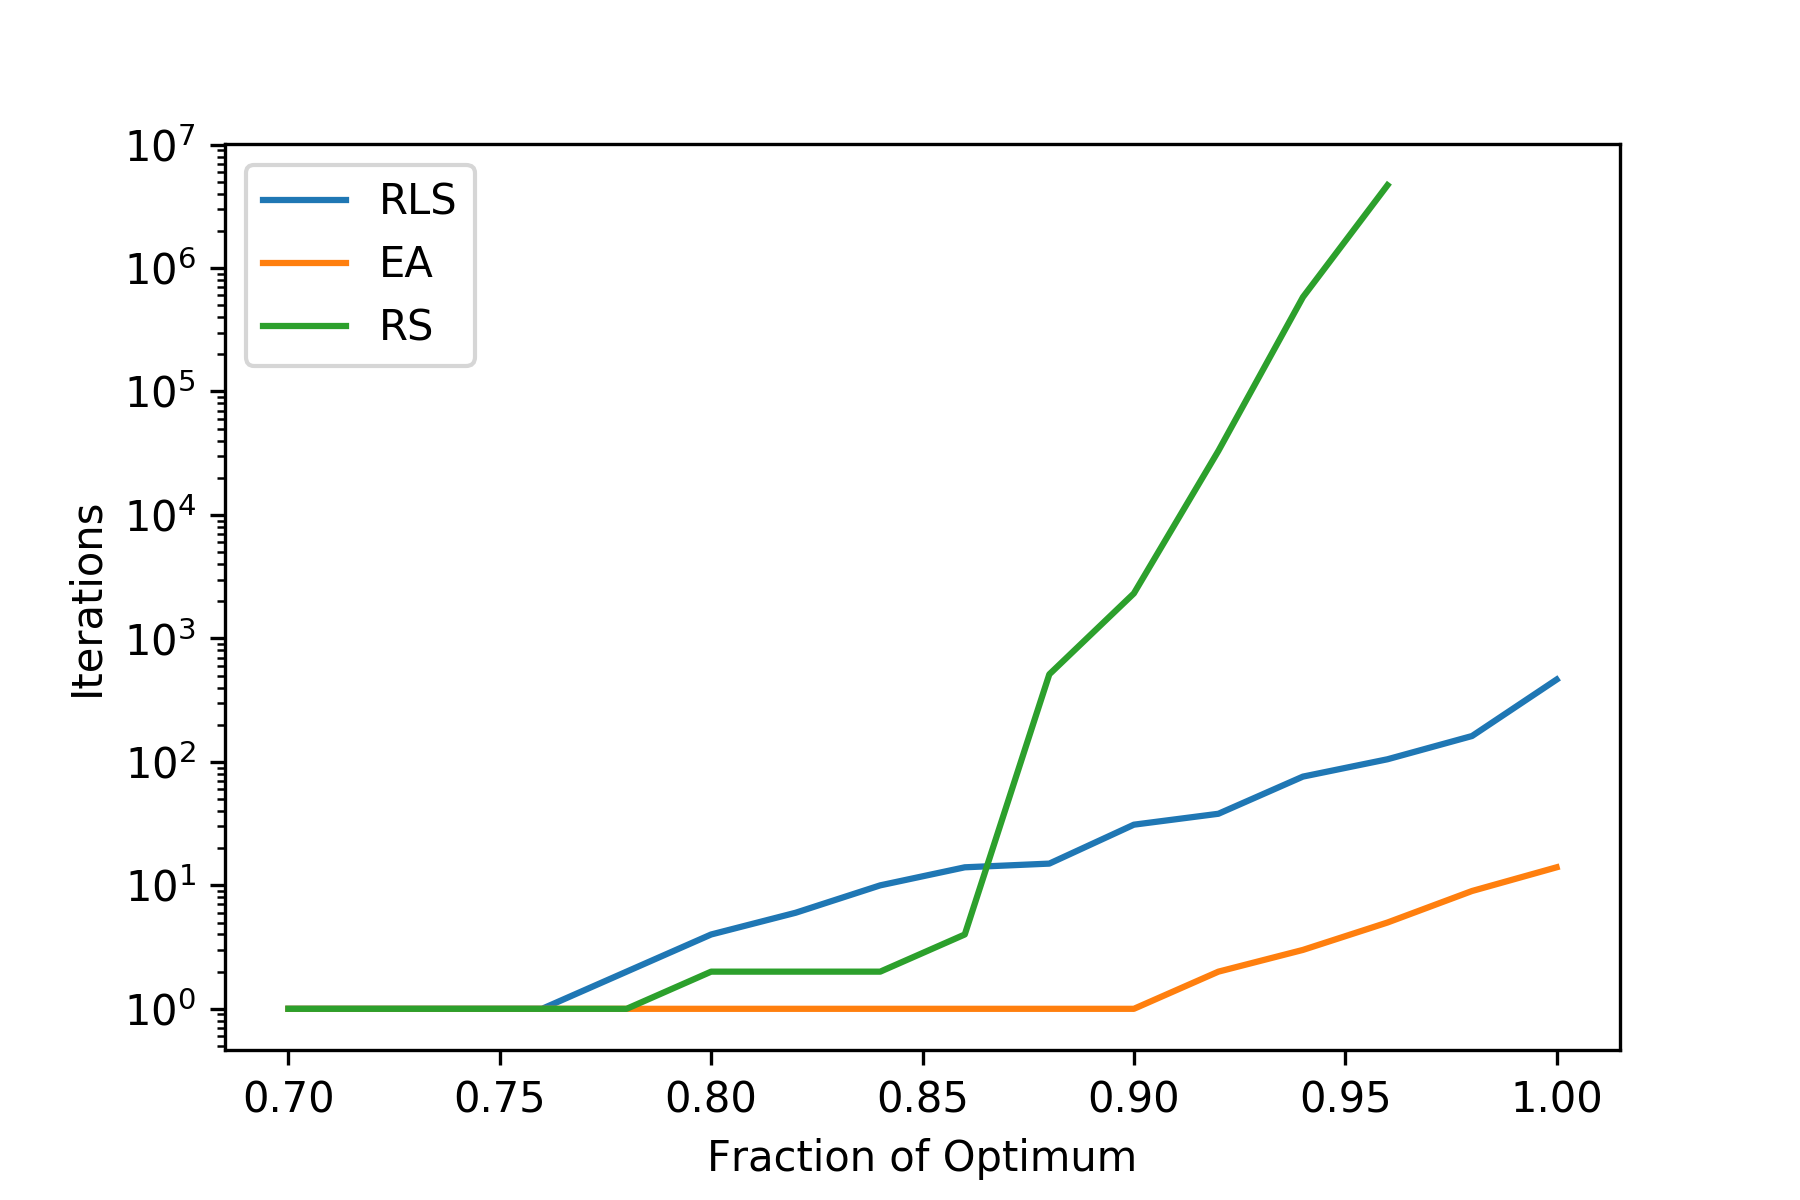
\includegraphics[width=\textwidth]{WT-16_T2.png}
    \caption{Comparison of needed iterations for the implemented algorithms to reach a certain fraction of the optimal solution for WT-16 with teaming 2.}
    \label{fig:wt_16}
\end{figure} 
 \end{center}
 
 In the beginning of this project, after implementing the fitness function, we started \textsc{RandomSearch} on four instances in parallel to search for the optimal student distribution for WT-15. After 300 hours we stopped the experiment. One instance found an individual with a score of 98.86\% of the optimal solution after 205 hours which equals 177 billion iterations. The remaining three instances found no better solution than 93.3\%, 93.6\%, and 95.7\% of the optimum within those 12 days of run time. In comparison, the evolutionary algorithm finds the optimal solution in only 100 iterations which equals roughly 30 seconds.
 
 \begin{center}
\begin{table}[]
\centering
\caption{Best results achieved by EA depending on semester for teaming 2}
\label{results_teaming2}
\begin{tabular}{l|l|l|l}
Semester & Lower Bound & Upper Bound & Best Result of EA \\ \hline
WT-15    & 10.27       & 43.83       & 43.83             \\ \hline
ST-16    & 9.49        & 42.55       & 42.17             \\ \hline
WT-16    & 10.40       & 45.08       & 45.07             \\ \hline
ST-17    & 9.32        & 42.20       & 41.54             \\
\end{tabular}
\end{table}
 \end{center}
 
\begin{center}
 \begin{table}[]
\centering
\caption{Best results achieved by EA depending on semester for teaming 3 and 4}
\label{results_teaming3_4}
\begin{tabular}{l|l|l}
\hline
Semester & Best Result for Teaming 3 & Best Result for Teaming 4 \\ \hline
WT-15    & 43.83                     & 43.83                     \\ \hline
ST-16    & 42.17                     & 42.17                     \\ \hline
WT-16    & 45.07                     & 45.07                     \\ \hline
ST-17    & 41.54                     & 41.52                     \\
\end{tabular}
\end{table}
\end{center}

As one can see in Table \ref{results_teaming2}, we are pretty confident to have found the optimal distribution of students for Winter Term 15 and Winter Term 16. Table \ref{results_teaming3_4} shows that the involvement of collisions only changed the fitness of the best individual found for Summer Term 17. Nevertheless, there were no collision in the best found teamings.\\
 
 From Figure \ref{fig:ea_iterations} we can tell that the different diversity measures for the teamings indeed influenced the average run time of the evolutionary algorithm. Overall, it appears that the algorithm needed more iterations to find the best solution if it was forced to minimize collisions that occurred easier. 
 
\begin{figure}[h]
    \centering
    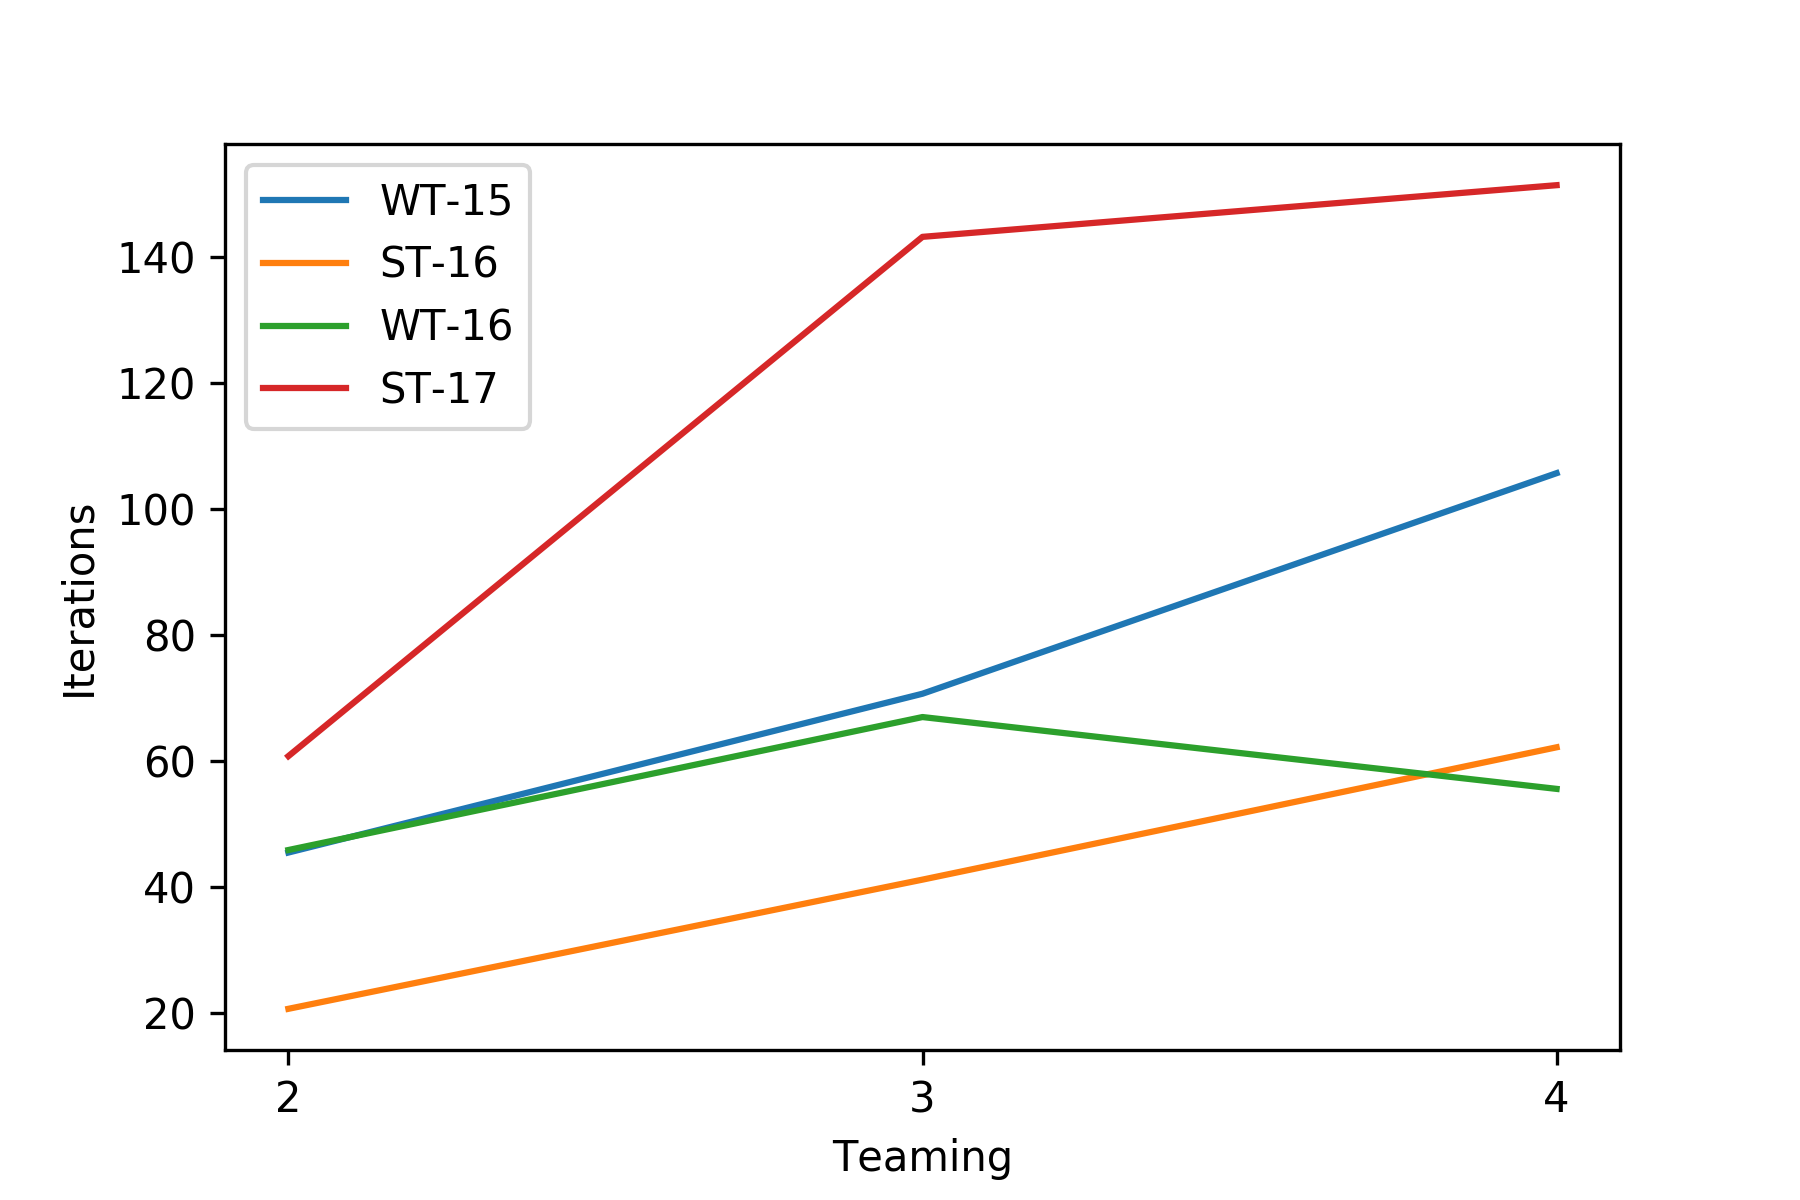
\includegraphics[width=0.7\textwidth]{EA_Iterations.png}
    \caption{Comparison of average iterations for the EA to find an optimum for the different teamings and semester.}
    \label{fig:ea_iterations}
\end{figure} 


\end{document}
